\section{Transformation des données}

\subsection{Les données dynamiques}

\subsubsection{Echelle}

Pour se rendre compte de la répartition des valeurs des données dynamiques, on affiche les histogramme de ces valeurs sur une echelle logarithmique:

\begin{figure}[H]
\captionsetup{labelformat=empty}
\minipage{0.50\textwidth}
  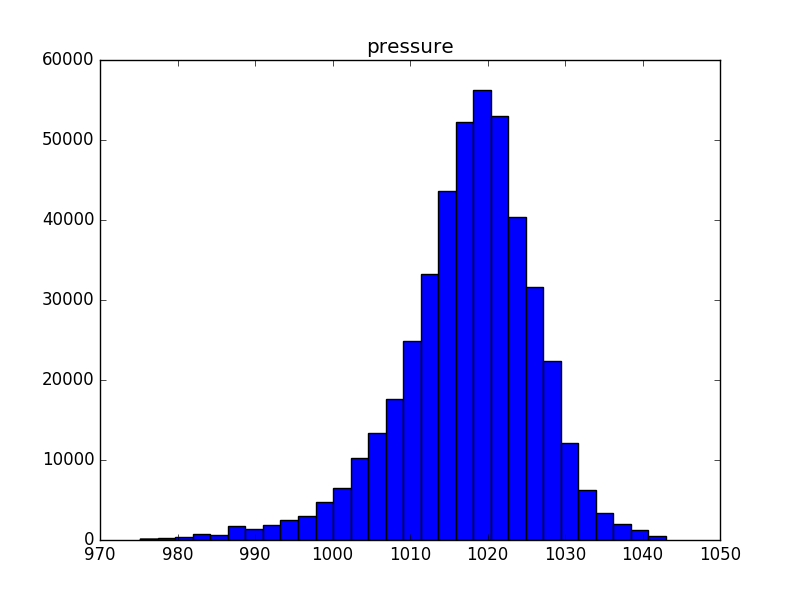
\includegraphics[width=\linewidth]{images/pression.png}
  \caption{pression}
\endminipage\hfill
\minipage{0.50\textwidth}
  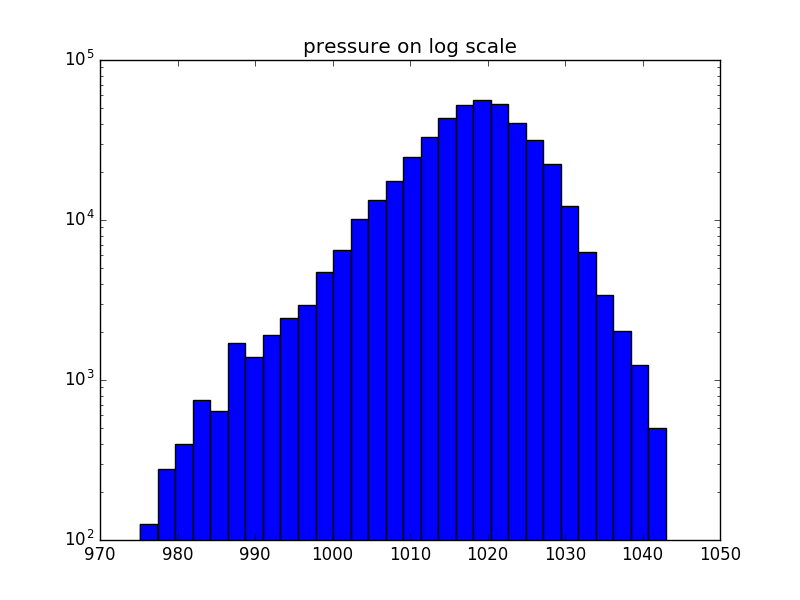
\includegraphics[width=\linewidth]{images/log_pression.png}
  \caption{pression sur échelle log}
\endminipage\hfill
\end{figure}

\begin{figure}[H]
\captionsetup{labelformat=empty}
\minipage{0.50\textwidth}
  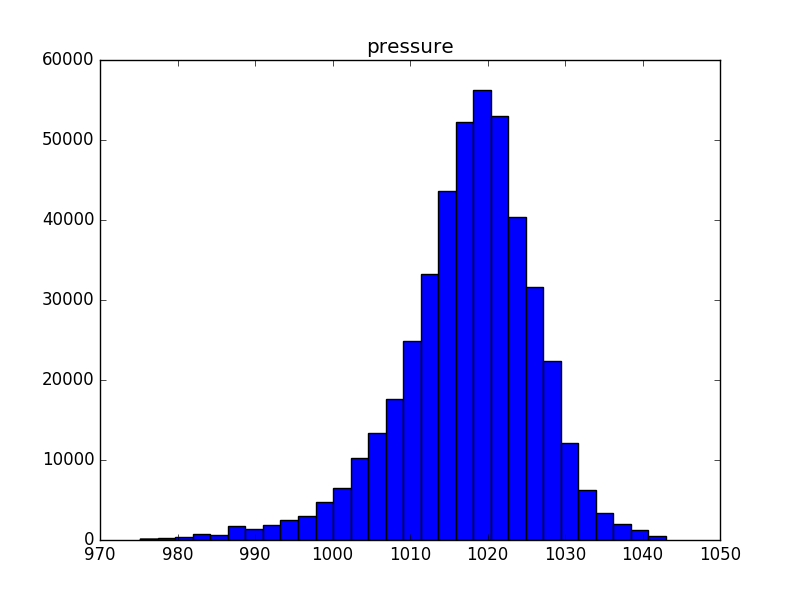
\includegraphics[width=\linewidth]{images/pression.png}
  \caption{pression}
\endminipage\hfill
\minipage{0.50\textwidth}
  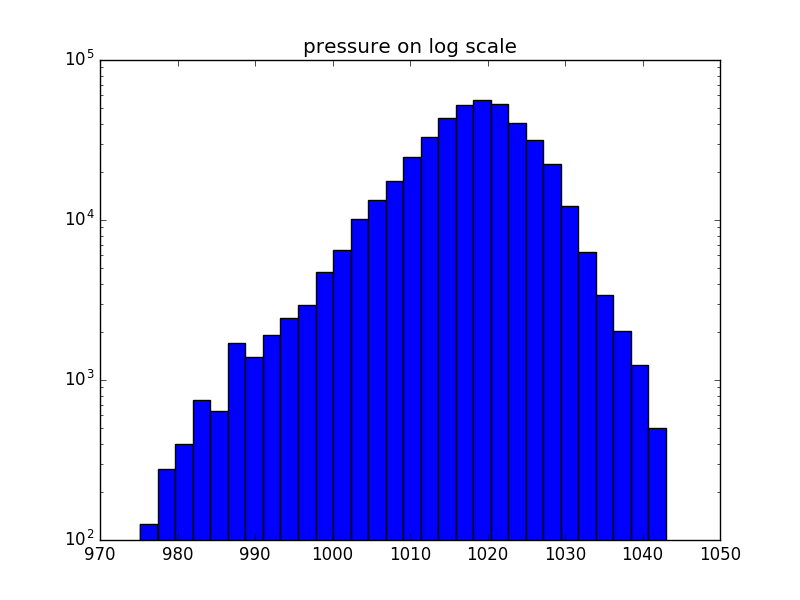
\includegraphics[width=\linewidth]{images/log_pression.png}
  \caption{pression sur échelle log}
\endminipage\hfill
\end{figure}

\begin{figure}[H]
\captionsetup{labelformat=empty}
\minipage{0.50\textwidth}
  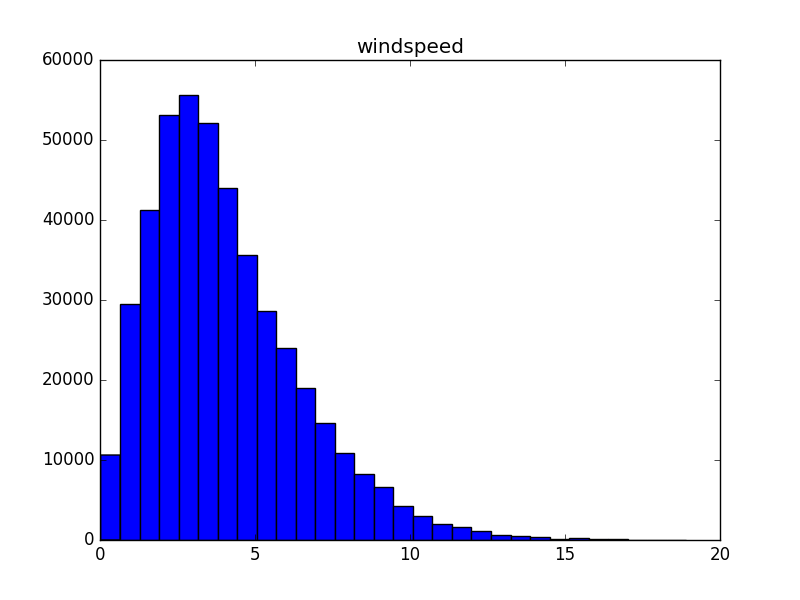
\includegraphics[width=\linewidth]{images/vent.png}
  \caption{vent}
\endminipage\hfill
\minipage{0.50\textwidth}
  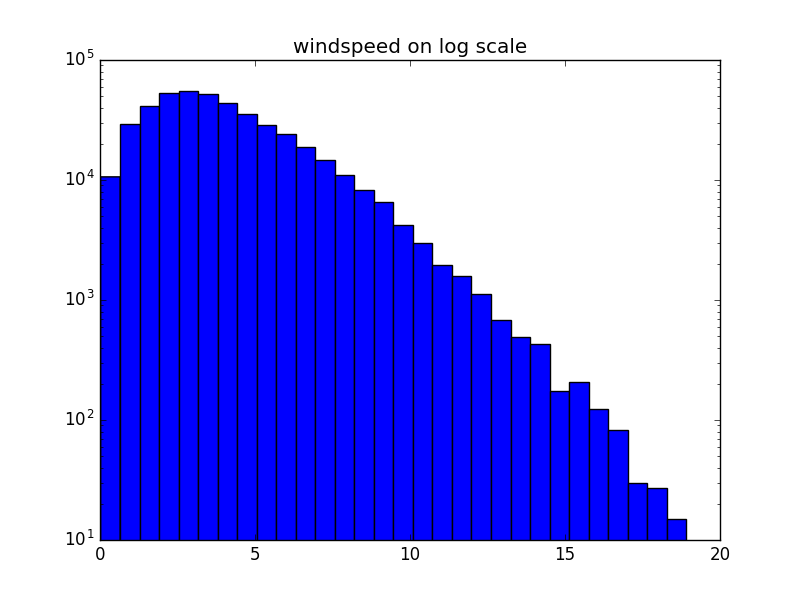
\includegraphics[width=\linewidth]{images/log_vent.png}
  \caption{vent sur échelle log}
\endminipage\hfill
\end{figure}

\begin{figure}[H]
\captionsetup{labelformat=empty}
\minipage{0.50\textwidth}
  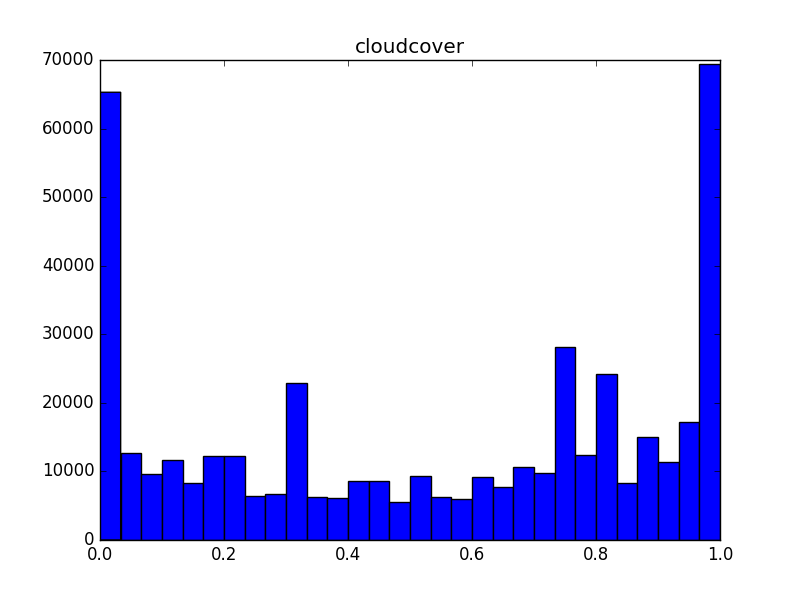
\includegraphics[width=\linewidth]{images/ennuagement.png}
  \caption{ennuagement}
\endminipage\hfill
\minipage{0.50\textwidth}
  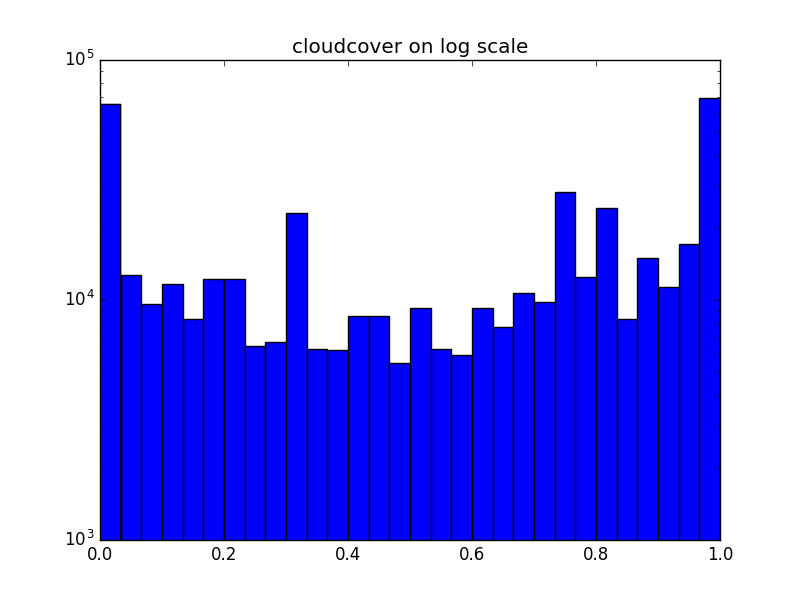
\includegraphics[width=\linewidth]{images/log_ennuagement.png}
  \caption{ennuagement sur échelle log}
\endminipage\hfill
\end{figure}

\begin{figure}[H]
\captionsetup{labelformat=empty}
\minipage{0.50\textwidth}
  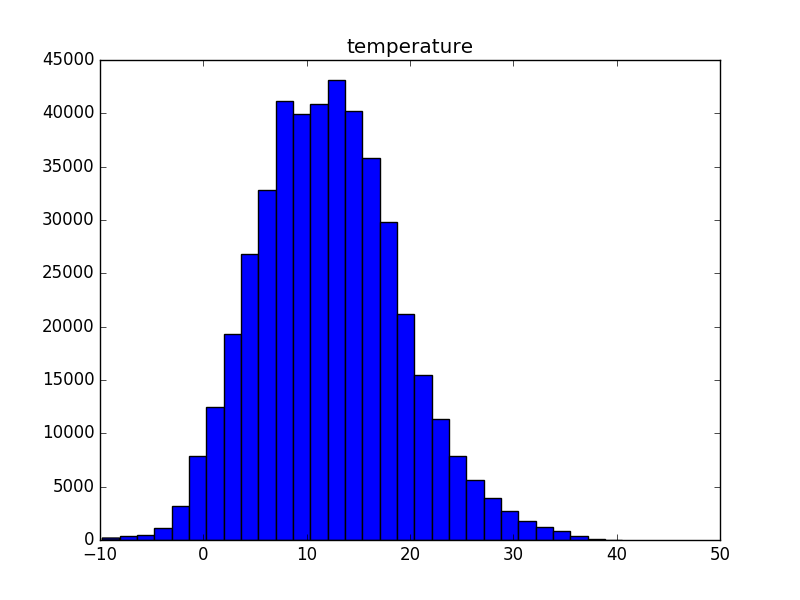
\includegraphics[width=\linewidth]{images/temperature.png}
  \caption{temperature}
\endminipage\hfill
\minipage{0.50\textwidth}
  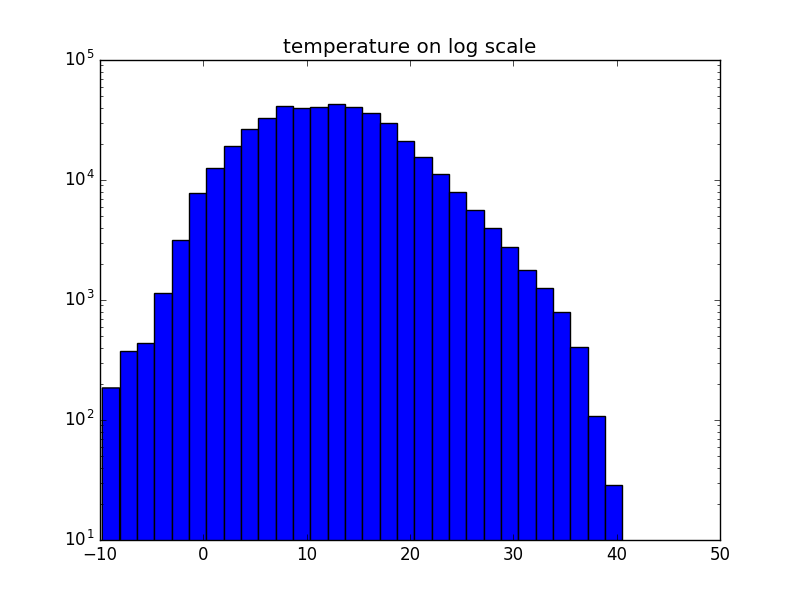
\includegraphics[width=\linewidth]{images/log_temperature.png}
  \caption{temperature sur échelle log}
\endminipage\hfill
\end{figure}

Il apparaît donc que les données sont plus étalées sur un échelles logarithmique.
Dans la mesure ou nous cherchons à appliques des techniques de régression simples et avec une forte régularité (regression lineaire), le fait d'utiliser des échelles logarithmiques est une première transformation que nous pouvons appliquer à nos données avant d'utiliser des modèles de régression simples.

\subsubsection{Représentations temps fréquence}

\subsection{Les données statiques}

Les données statiques sont des surfaces cumulées dans des périmètres de plus en plus grands

